\documentclass[12pt]{exam}
\usepackage{amsmath, amssymb}
\usepackage{booktabs, tabularx} % For text alignment on cover page
\usepackage{epsfig}             % For \includegraphics command

\newcolumntype{C}{>{\centering\arraybackslash}X}

\begin{document}
\addpoints
\setlength{\parindent}{0cm}

\begin{center}

{\Large\textbf{MATH 040 - Midterm}}\\
\medskip
{\Large{Spring 2020}}

\vskip1cm
\makebox[0.7\textwidth]{\large Last Name:\enspace\hrulefill}
\vskip0.4cm
\makebox[0.7\textwidth]{\large First Name:\enspace\hrulefill}
\vskip0.4cm

\makebox[0.7\textwidth]{\large Signature:\enspace\hrulefill}
\vskip0.4cm

\end{center}
\bigskip
\textbf{Instructions:}
\begin{itemize}
  \item Please put away notes, and turn off and put away phones.
  \item Basic calculators are permitted.
  \item Ask me if you have any questions about what a problem is asking.
\end{itemize}
\vskip0.4cm
\begin{center}
  \gradetable[h][questions]
\end{center}

\newpage
\vskip1cm

%
\begin{questions}
% \pointformat{}
\pagebreak

\question[6] {
  True or false. \begin{parts}
    \item $\displaystyle \frac{4}{5} > \frac{41}{50}$
    \\~\\
    \item $\displaystyle \frac{3}{4} < 0.8$
    \\~\\
    \item $\displaystyle (-2)^6 > -2^6$
    \\~\\
  \end{parts}
}

\question[6] {
  Evaluate the following expressions \begin{parts}
    \item $a^3 + a^2$ when $a = -2$
    \\~\\~\\~\\
    \item $\displaystyle\left(\frac{1}{2}d\right)^2$ when $d = 6$
    \\~\\~\\~\\
    \item $\displaystyle \left(\frac{1}{x}\right)^3$ when $x = 10$
    \\~\\~\\~\\
  \end{parts}
}
\pagebreak

\question[10] {
  Suppose you just got two offers for sales jobs. \begin{enumerate}
    \item[(A)] In job A, you will earn a base salary of $\$5000$ each month,
    plus $6\%$ of sales in commission.
    \item[(B)] In job B, you will earn a base salary of $\$4000$ each month,
    plus $10\%$ of sales in commission.
  \end{enumerate}
  Set up a linear inequality that describes the amount of sales that you'll have
  to do each month in order to make more money with the second job than with the
  first, where the variable $x$ denotes sales in dollars. Solve for $x$.
}
\pagebreak
\question[12] {
  Suppose that the number of baseball cards that Alex owns is given by ${y = 200 + 6x}$
  where $x$ is the number of months since Alex's 12th birthday.
  \begin{parts}
    \item What is the value of the slope in this equation, and what does it represent in terms of baseball cards?
    \item What is the value of the $y$-intercept, and what does it represent in
    terms of baseball cards?
    \item How many baseball cards does Alex own on her 13th birthday?
    (Hint: recall that $x$ represents the number of \textit{months} since her 12th birthday.)
  \end{parts}
}
\pagebreak
\question[10] {
  Suppose you are a farmer with $100$ meters of fencing that you plan to use to
  enclose a $10$ meter by $\ell$ meter section of your grass lot. The enclosed area
  needs to have at least $350$ square meters of space for your animals.
  Find \textbf{all} values of $\ell$ such that the perimeter no more than $100$
  meters while the area of the lot is at least 350 square meters?
  \\~\\
  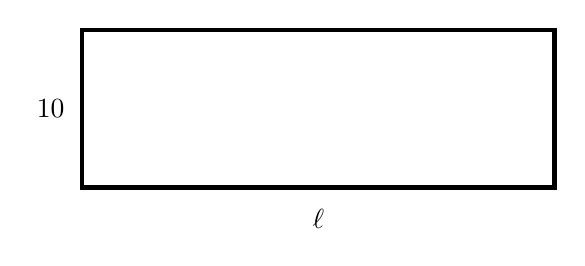
\begin{tikzpicture}[scale=2]
    \draw[ultra thick] (0,0) rectangle (3, 1);
    \node at (-0.2, 0.5) {$10$};
    \node at (1.5, -0.2) {$\ell$};
  \end{tikzpicture}
}
\pagebreak
\question[12] {
  Consider the function $f(x) = |2x| - 1$.
  \begin{parts}
    \part Compute
      \begin{enumerate}[(i)]
        \item $f(-1)$
        \item $f(-\frac12)$
        \item $f(0)$
        \item $f(2)$
      \end{enumerate}
    \part Graph the function $f$ including the four points above.
    \\~\\
    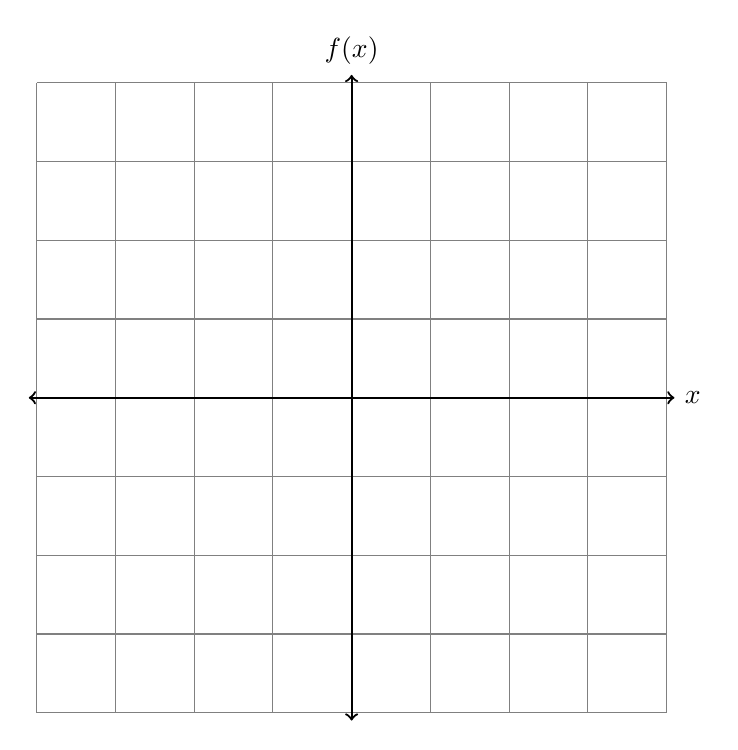
\begin{tikzpicture}
      \draw[gray] (-4,-4) grid (4, 4);
      \draw[thick,<->] (-4.1,0)--(4.1,0) node[right] {$x$};
      \draw[thick,<->] (0,-4.1)--(0,4.1) node[above] {$f(x)$};
    \end{tikzpicture}
    \part What is the domain of the function $f$?
    \\~\\~\\~\\
    \part What is the range of the function $f$?
  \end{parts}
}
\pagebreak
\question[12] {
  At a 2018 basketball tournament, tickets cost $\$10$ for adults and $\$5$ for children.
  Suppose 300 people came to the game, and ticket sales totaled $\$2400$.
  Set up a system of equations and use it to determine how many of the attendees were children.
}
\pagebreak
\question[12] {
  Suppose that a toy company has learned that if they price a toy at $\$3$, they
  will sell $1000$ units, and if they price a toy at $\$4$, they will sell $700$
  units.
  \begin{parts}
    \part Assuming that the price-sales relationship is linear, write a linear
    equation describing the number of units sold as a function of price.
    \part If the company gives away toys for free, how many will they give away
    according to this linear model?
  \end{parts}
}
\end{questions}
\end{document}
